% !TEX root = saveliev_physics_general_course_2.tex
%!TEX TS-program = pdflatex
%!TEX encoding = UTF-8 Unicode

\chapter[INTERACTION OF ELECTROMAGNETIC WAVES WITH A \\ SUBSTANCE]{INTERACTION OF \\ ELECTROMAGNETIC \\ WAVES WITH A SUBSTANCE}\label{chap:20}
\chaptermark{INTERACTION OF ELECTROMAGNETIC WAVES WITH A SUBSTANCE}

\section{Dispersion of Light}\label{sec:20_1}

By the \textbf{dispersion of light} are meant phenomena due to the dependence of the refractive index of a substance on the length of the light
wave.
This dependence can be characterized by the function
\begin{equation}\label{eq:20_1}
    n = f(\lambda_0),
\end{equation}

\noindent
where $\lambda_0$ is the length of a light wave in a vacuum.

The derivative of $n$ with respect to $\lambda_0$ is called the \textbf{dispersion of a substance}.

Function \eqref{eq:20_1} for all transparent colourless substances in the visible part of the spectrum has the nature shown in \fig{20_1}.
Diminishing of the wavelength is attended by an increase in the refractive index at a constantly growing rate.
Hence, the dispersion of a substance $\diffin{n}{\lambda_0}$ is negative.
Its absolute value increases when $\lambda_0$ decreases.

If a substance absorbs part of the rays, then the course of dispersion displays an anomaly in the region of absorption and near it (see \fig{20_6}).
On a certain section, the dispersion of the substance $\diffin{n}{\lambda_0}$ will be positive.
Such a variation of $n$ with $\lambda_0$ is called
\textbf{anomalous dispersion}.

Media having the property of dispersion are known as \textbf{dispersing} ones.
In these media, the speed of light waves depends on the wavelength $\lambda_0$ or the frequency $\omega$.

\begin{figure}[t]
	\begin{center}
		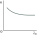
\includegraphics[scale=1]{figures/ch_20/fig_20_1.pdf}
		% \caption[]{}
        \caption[]{Dispersion curve of a substance for all transparent colourless substances in the visible part of the spectrum.}
		\label{fig:20_1}
	\end{center}
	\vspace{-0.8cm}
\end{figure}

\section{Group Velocity}\label{sec:20_2}

Strictly monochromatic light of the kind
\begin{equation}\label{eq:20_2}
	E = A \cos(\omega t - k x + \alpha)
\end{equation}

\noindent
is an infinite sequence in time and space of ``crests'' and ``valleys'' propagating along the $x$-axis with the phase velocity
\begin{equation}\label{eq:20_3}
	v = \frac{\omega}{k}
\end{equation}

\noindent
[see \eqn{19_4}].
We cannot use such a wave to transmit a signal because each following crest differs in no way from the preceding one.
To transmit a signal, we must put a ``mark'' on the wave, say, interrupt it for a certain time $\Delta t$.
In this case, however, the wave will no longer be described by \eqn{20_2}.

It is the simplest to transmit a signal with the aid of a light pulse (\fig{20_2}).
According to the Fourier theorem, such a pulse can be represented as the superposition of waves of the kind given by \eqn{20_2} having frequencies confined within a certain interval $\Delta\omega$.
A superposition of waves differing only slightly from one another in frequency is called a \textbf{wave packet} or a \textbf{wave group}.
The analytical expression for a wave packet has the form
\begin{equation}\label{eq:20_4}
	E(x,t) = \int_{\omega_0-\Delta\omega/2}^{\omega_0+\Delta\omega/2} A_{\omega} \cos(\omega t - k_{\omega} x + \alpha_{\omega})\, \deriv{\omega}
\end{equation}

\noindent
(the subscript $\omega$ used with $A$, $k$, and $\alpha$ indicates that these quantities differ for different frequencies).
With a fixed value of $t$, a plot of function \eqref{eq:20_4} has the form shown in \fig{20_2}.
When $t$ changes, the graph becomes displaced along the $x$-axis.
Within the limits of a packet, plane waves amplify one another to a greater or smaller extent.
Outside these limits, they virtually completely annihilate one another.

\begin{figure}[t]
	\begin{center}
		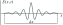
\includegraphics[scale=1]{figures/ch_20/fig_20_2.pdf}
		% \caption[]{}
        \caption[]{Light pulse for transmitting a signal, \eqn{20_4}, with a fixed value of $t$. When t changes, the graph becomes displaced along the $x$-axis. Within the limits of a packet, plane waves amplify one another to a greater or smaller extent. Outside these limits, they virtually completely annihilate one another.}
		\label{fig:20_2}
	\end{center}
	\vspace{-0.8cm}
\end{figure}

The relevant calculations show that the smaller the width of a packet $\Delta{x}$, the greater is the interval of frequencies $\Delta{\omega}$ or accordingly the greater is the interval of wave numbers $\Delta{k}$ needed to describe a packet with the aid of \eqn{20_4}.
The following relation holds:
\begin{equation}\label{eq:20_5}
	\Delta{k} \Delta{x} \approx 2\pi.
\end{equation}

We must stress the fact that for the superposition of waves described by \eqn{20_4} to be considered a wave packet, the condition $\Delta{\omega}\ll\omega_0$ must be obeyed.

In a non-dispersing medium, all the plane waves forming a packet propagate with the same phase velocity $v$.
It is evident that in this case the velocity of the packet coincides with $v$, and the shape of the
packet does not change with time.
It can he shown that a packet spreads in a dispersing medium with time---its width grows.
If the dispersion is not great, spreading of the packet is not too fast.
In this case, we can say that the packet travels with the velocity $u$, by which we mean the velocity of the centre of the packet, \ie, of the point with the maximum value of $E$.
This velocity is called the \textbf{group velocity}.
In a dispersing medium, the group velocity $u$ differs from the phase velocity $v$ (here we mean the phase velocity of the harmonic component with the maximum amplitude, in other words, the phase velocity for the dominating frequency).
We shall show below that when $\diffin{n}{\lambda_0}<0$, the group velocity is smaller than the phase one ($u<v$); when $\diffin{n}{\lambda_0}>0$, the group velocity is greater than the phase one ($u>v$).

Figure \ref{fig:20_3} shows ``photographs'' of a wave packet for three consecutive moments $t_1$, $t_2$, and $t_3$.
The figure is for the case when $u<v$.
Inspection of the figure shows that motion of the packet is attended by motion of the crests and valleys ``inside'' it.
New crests constantly appear at the left-hand boundary of the packet.
After travelling along the packet, they vanish at its right-hand boundary.
Hence, whereas the packet as a whole travels with the velocity $u$, the individual crests and valleys travel with the velocity $v$.

\begin{figure}[t]
	\begin{center}
		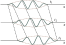
\includegraphics[scale=1]{figures/ch_20/fig_20_3.pdf}
		% \caption[]{}
        \caption[]{``Photographs'' of a wave packet for three consecutive moments $t_1$, $t_2$, and $t_3$, for $u<v$. The motion of the packet is attended by motion of the crests and valleys ``inside'' it. New crests constantly appear at the left-hand boundary of the packet. After travelling along the packet, they vanish at its right-hand boundary. Hence, whereas the packet as a whole travels with the velocity $u$, the individual crests and valleys travel with the velocity $v$.}
		\label{fig:20_3}
	\end{center}
	\vspace{-0.8cm}
\end{figure}

When $u>v$, the directions of motion of the packet and of the crests inside it are opposite.

Let us explain what has been said above using the example of the superposition of two plane waves of the same amplitude and of different wavelengths $\lambda$.
Figure \ref{fig:20_4} gives an ``instant photograph'' of the waves.
One of them is shown by a solid line, and the other by a dash line.
The intensity is the greatest at point A where the phases of the two waves coincide at the given moment.
At points B and C, the two waves are in counterphase, owing to which the intensity of the
resultant wave is zero.
Assume that both waves are propagating from left to right, the velocity of the ``solid'' wave being lower than that of the ``dash'' one (here $\diffin{n}{\lambda}>0$ and, consequently, $\diffin{n}{\lambda}<0$).

Thus, the place at which the waves amplify each other will move to the left with time relative to the waves.
As a result, the group velocity will be lower than the phase value.
If the velocity of the ``solid'' wave is greater than that of the "dash" one (\ie, $\diffin{n}{\lambda}>0$), the place at which amplification of the waves occurs will move to the right so that the group velocity will be greater than the phase one.

Let us write the equations of the waves, assuming for simplicity that the initial phases equal zero:
\begin{align*}
	E_1 &= A \cos(\omega t - k x)\\
	E_2 &= A \cos[(\omega+\Delta{\omega}) t - (k+\Delta{k}) x].
\end{align*}

Here $k=\omega/v_1$, and $(k+\Delta{k}) = (\omega+ \Delta{\omega})/v_2$.
Assume that $\Delta{\omega}\ll\omega$, hence, $\Delta{k}\ll k$.
Now, summating the oscillations and performing transformations according to the formula for the sum of cosines, we get
\begin{equation}\label{eq:20_6}
	E = E_1 + E_2 = \bracket{2A\cos\parenthesis{\frac{\Delta\omega}{2} t - \frac{\Delta{k}}{2}x}} \cos(\omega t - kx)
\end{equation}

\noindent
(in the second multiplier, we have disregarded $\Delta{\omega}$ in comparison with $\omega$ and $\Delta{k}$ in comparison with $k$).

\begin{figure}[t]
	\begin{center}
		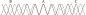
\includegraphics[scale=1]{figures/ch_20/fig_20_4.pdf}
		% \caption[]{}
        \caption[]{``Instant photograph'' of two waves. The intensity is the greatest at point A where the phases of the two waves coincide at the given moment. At points B and C, the two waves are in counterphase, owing to which the intensity of the resultant wave is zero.}
		\label{fig:20_4}
	\end{center}
	\vspace{-0.8cm}
\end{figure}

The multiplier in brackets varies much more slowly with $x$ and $t$ than the second multiplier.
We can therefore consider expression \eqref{eq:20_6} as the equation of a plane wave whose amplitude varies according to the law\footnote{Compare with Eqs. (7.86) and (7.87) of Vol. I. The dependence of function \eqref{eq:20_6} on $x$ at a fixed value of $t$ is depicted by a curve similar to the one in Fig. 7.11a of Vol. 1.}
\begin{equation*}
	\text{Amplitude } = \absolute{2A\cos\parenthesis{\frac{\Delta\omega}{2} t - \frac{\Delta{k}}{2}x}}.
\end{equation*}

\noindent
In the given case, there is a number of identical amplitude maxima determined by the condition
\begin{equation}\label{eq:20_7}
	\frac{\Delta{\omega}}{2} t - \frac{\Delta{k}}{2} \ab{x}{max} = \pm m \pi \quad (m = 0,1,2,\ldots).
\end{equation}

\noindent
Each of these maxima can be considered as the centre of the relevant wave packet.

Solving \eqn{20_7} relative to $\ab{x}{max}$ we get
\begin{equation*}
	\ab{x}{max} = \frac{\Delta{\omega}}{\Delta{k}} t + \text{constant}.
\end{equation*}

\noindent
It thus follows that the maxima travel with the velocity
\begin{equation}\label{eq:20_8}
	u = \frac{\Delta{\omega}}{\Delta{k}}.
\end{equation}

\noindent
The expression obtained is the group velocity for a packet formed by two components.

Let us find the velocity with which the centre of a wave packet described by expression \eqref{eq:20_5} travels.
Passing over from cosines to exponents, we get
\begin{equation}\label{eq:20_9}
	E(x,t) = \int_{\omega_0-\Delta\omega/2}^{\omega_0+\Delta\omega/2} \hat{A}_{\omega} \exp[i(\omega t - k_{\omega}x)]\, \deriv{\omega}
\end{equation}

\noindent
[$\hat{A}_{\omega} = A_{\omega}\exp(i\alpha_{\omega})$ is the complex amplitude].

Let us expand the function $k_{\omega}=k(\omega)$ into a series in the vicinity of $\omega_0$:
\begin{equation}\label{eq:20_10}
	k_{\omega} = k_0 + \parenthesis{\diff{k}{\omega}}_0 (\omega - \omega_0) + \ldots .
\end{equation}

\noindent
Here, $k_0=k(\omega)_0$, and $(\diffin{k}{\omega})_0$ is the value of the derivative at point $\omega_0$.

We shall introduce the variable $\xi=\omega-\omega_0$.
Hence, $\omega=\omega_0+\xi$ and $\deriv{\omega} = \deriv{t}$.
Performing such a substitution in \eqn{20_9} and introducing the value of $k_{\omega}$ from \eqn{20_10}, we can write
\begin{equation}\label{eq:20_11}
	E(x,t) = \exp[i(\omega_0 t - k_0 x)] \int_{-\Delta\omega/2}^{+\Delta\omega/2} \hat{A}_{\xi} \exp\bracet{i \bracket{ t - \parenthesis{\diff{k}{\omega}}_0 x } \xi}\, \deriv{\xi}.
\end{equation}

\noindent
We have arrived at an equation of a plane wave of frequency $\omega_0$, wave number $k_0$, and complex amplitude
\begin{equation}\label{eq:20_12}
	\hat{A}(x,t) = \int_{-\Delta\omega/2}^{+\Delta\omega/2} \hat{A}_{\xi} \exp\bracet{i \bracket{ t - \parenthesis{\diff{k}{\omega}}_0 x } \xi}\, \deriv{\xi}.
\end{equation}

\noindent
It can be seen from \eqn{20_12} that the equation
\begin{equation}\label{eq:20_13}
	t - \parenthesis{\diff{k}{\omega}}_0 x = \text{constant},
\end{equation}

\noindent
relates the time $t$ and the coordinate $x$ of the plane in which the complex amplitude has a given fixed value, in particular including a value such that the magnitude of the complex amplitude, \ie, the conventional amplitude $A(x,t)$, reaches a maximum.

Taking into account that $1/(\diffin{k}{\omega})_0 = (\diffin{\omega}{k})_0$, we can write \eqn{20_13} in the form
\begin{equation}\label{eq:20_14}
	\ab{x}{max} = \parenthesis{\diff{k}{\omega}}_0 t - \text{constant}' \quad \bracket{\text{constant}'=\frac{\text{constant}}{(\diffin{k}{\omega})_0}}.
\end{equation}

It follows from \eqn{20_14} that the place where the amplitude of a wave packet is maximum travels with the velocity $(\diffin{\omega}{k})_0$.
We thus arrive at the following expression for the group velocity:
\begin{equation}\label{eq:20_15}
	u = \diff{\omega}{k}
\end{equation}

\noindent
(the subscript $0$ is no longer needed and has been omitted).
We previously obtained a similar expression for a packet of two waves [see \eqn{20_8}].
We remind our reader that we have disregarded the terms of higher orders of smallness in expansion \eqref{eq:20_8}.
In this approximation, the shape of the wave packet does not change with time.
If we take into account the following terms of the expansion, then we get an expression for the amplitude from which it follows that the width of a packet grows with time---a wave packet broadens.

We can give a different form to the expression for the group velocity.
Substituting $vk$ for $\omega$ [see \eqn{20_3}], we can write \eqn{20_14} as follows:
\begin{equation}\label{eq:20_16}
	u = \diff{(vk)}{k} = v + k \diff{v}{k}.
\end{equation}

\noindent
We shall further write
\begin{equation*}
	\diff{v}{k} = \diff{v}{\lambda} \diff{\lambda}{k}.
\end{equation*}

We find from the relation $\lambda = 2\pi/k$ that $\diffin{\lambda}{k}=-2\pi/k^2=-\lambda/k$.
Accordingly, $\diffin{v}{k}=-(\diffin{v}{\lambda}) (\lambda/k)$.
Using this value in \eqn{20_16}, we get
\begin{equation}\label{eq:20_17}
	u = v - \lambda \diff{v}{\lambda}.
\end{equation}

\noindent
A glance at this formula shows that the group velocity $u$ can be either smaller or greater than the phase velocity $v$, depending on the sign of $\diffin{v}{\lambda}$.
In the absence of dispersion, $\diffin{v}{\lambda} = 0$, and the group velocity coincides with the phase one.

The maximum of the intensity falls to the centre of a wave packet.
Therefore, when the concept of group velocity has a meaning, the velocity of energy transfer by a wave equals the group velocity.

\textit{The concept of group velocity may be applied only provided that the absorption of the wave energy in the given medium is not great.}
With considerable attenuation of the waves, the concept of group velocity loses its meaning.
This occurs in the region of anomalous dispersion.
In this region, the absorption is very great, and the concept of group velocity cannot be applied.

\section{Elementary Theory of Dispersion}\label{sec:20_3}

The dispersion of light can be explained on the basis of the electromagnetic theory and the electron theory of a substance.
For this purpose, we must consider the process of interaction of light with a substance.
The motion of the electrons in an atom obeys the laws of quantum mechanics.
In particular, the concept of the trajectory of an electron in an atom loses all meaning.
As Lorentz showed, however, it is sufficient to restrict ourselves to the hypothesis on the existence of electrons bound quasi-elastically within atoms for a qualitative understanding of many optical phenomena.
When brought out of their equilibrium position, such electrons will begin to oscillate, gradually losing the energy of oscillation on the emission of electromagnetic waves.
As a result, the oscillations will be damped.
The attenuation can be taken into account by introducing the ``force of friction of emission'' proportional to the velocity.

When an electromagnetic wave passes through a substance, every electron experiences the action of the Lorentz force
\begin{equation}\label{eq:20_18}
	\vec{F} = -e \vec{E} - e (\vecprod{v}{B}) = -e \vec{E} - e\mu_0 (\vecprod{v}{H})
\end{equation}

\noindent
[see \eqn{6_35}; the charge of an electron is $-e$].
According to \eqn{15_23}, the ratio of the magnetic and electric field strengths in a wave is $H/E = \sqrt{\varepsilon_0/\mu_0}$.
Hence, from \eqn{20_18}, we get the following value for the ratio of the magnetic and electric forces exerted on an electron
\begin{equation*}
	\frac{\mu_0 v H}{E} = \mu_0 v \parenthesis{\frac{\varepsilon_0}{\mu_0}}^{1/2} = v \sqrt{\varepsilon_0\mu_0} = \frac{v}{c}.
\end{equation*}

\noindent
Even if the amplitude $a$ of electron oscillations reached a value of the order of \SI{1}{\angstrom} (\SI{e-10}{\metre}), \ie, of the order of an atom's dimensions, the amplitude of the velocity of an electron $a\omega$ would be about $\num{e-10}\times\num{3e15}=\SI{3e5}{m.s^{-1}}$ [according to \eqn{16_6}, $\omega = 2\pi \nu$ equals about \SI{3e15}{rad.s^{-1}}].
Thus, the ratio $v/c$ is clearly less than \num{e-3} so that we may disregard the second addend in \eqn{20_18}.

We can thus consider that when an electromagnetic wave passes through a substance, every electron experiences the force
\begin{equation*}
	F = -e E_0 \cos(\omega t + \alpha)
\end{equation*}

\noindent
($\alpha$ is a quantity determined by the coordinates of a given electron, and $E_0$ is the amplitude of the electric field strength of the wave).

To simplify our calculations, we shall first disregard the attenuation due to emission.
We shall subsequently take the attenuation into account by introducing the relevant corrections into the formulas obtained.
The equation of motion of an electron in this case has the form
\begin{equation*}
	\ddot{r} + \omega_0^2 r = -\frac{e}{m} E_0 \cos(\omega t + \alpha)
\end{equation*}

\noindent
[see Eq. (7.13) of Vol. I,]; $\omega_0$ is the natural frequency of oscillations of an electron).
Let us add $-i(e/m)E_0\sin(\omega t+\alpha)$ to the right-hand side of this equation and thus pass over to the complex functions $\hat{E}$ and $\hat{r}$:
\begin{equation}\label{eq:20_19}
	\diffsec{\hat{r}}{t} + \omega^2 \hat{r} = -\frac{e}{m} \hat{E}_0 \exp(i\omega t).
\end{equation}

Here, $\hat{E}_0=E_0\exp(i\alpha)$ is the complex amplitude of the electric field of a wave.

We shall seek a solution of the equation in the form $\hat{r}=\hat{r}_0\exp(i\omega t)$, where $\omega$ is the complex amplitude of oscillations of an electron.
Accordingly, $\diffsecin{\hat{r}}{t}=-\omega^2 \hat{r}_0\exp(i\omega t)$.
Introducing these expressions into \eqn{20_19} and cancelling out the common factor $\exp(i\omega t)$, we arrive at the expression
\begin{equation*}
	-\omega^2 \hat{r}_0 + -\omega_0^2 \hat{r}_0 = -\frac{e}{m} \hat{E}_0,
\end{equation*}

\noindent
whence
\begin{equation*}
	\hat{r}_0 = \frac{-(e/m) \hat{E}_0}{(\omega_0^2-\omega^2}.
\end{equation*}

\noindent
Multiplying the equation obtained by $\exp(i\omega t)$, we obtain
\begin{equation*}
	\hat{r}(t) = \frac{-(e/m) \hat{E}(t)}{(\omega_0^2-\omega^2}.
\end{equation*}

\noindent
Finally, taking the real parts of the complex functions $\hat{r}$ and $\hat{E}$, we find $r$ as a function of $t$:
\begin{equation}\label{eq:20_20}
	r(t) =\frac{-(e/m) E(t)}{(\omega_0^2-\omega^2}.
\end{equation}

To simplify the problem, we shall consider that the molecules are non-polar.
In addition, since the masses of nuclei are great in comparison with the mass of an electron, we shall ignore the displacements of the nuclei from the equilibrium positions under the action of the wave field.
In this approximation, the dipole electric moment of a molecule can be represented in the form
\begin{align*}
	\vec{p}(t) &= \sum_l q_l \vec{R}_{0,l} + \sum_k e_k [\vec{r}_{0,k} + \vec{r}_k(t)]\\
	&= \bracet{ \sum_l q_l \vec{R}_{0,l} + \sum_k e_k \vec{r}_{0,k} } + \sum_k e_k \vec{r}_k(t)\\
	&= \vec{p}_0 + \sum_k e_k \vec{r}_k(t) = \sum_k e_k \vec{r}_k(t),
\end{align*}

\noindent
where $q_l$ and $R_{0,l}$ are the charges and position vectors of the equilibrium positions of the nuclei, $e_k$ and $r_{0,k}$ are the charge and position vector of the equilibrium position of the $k$-th electron, $\vec{r}_k(t)$ is the displacement of the $k$-th electron from its equilibrium position under the action of the wave
field, and $\vec{p}_0$ is the dipole moment of a molecule in the absence of a field, which is assumed to equal zero.

All the $\vec{r}_k(t)$'s are collinear with $\vec{E}(t)$.
We therefore obtain the following expression for the projection of $\vec{p}(t)$ onto the direction
of $\vec{E}(t)$:
\begin{equation*}
	p(t) = \sum_k e_k r_k(t) = \sum_k (-e) r_k(t)
\end{equation*}

\noindent
(we have taken into account that $e_k$ for all electrons is identical and equals $-e$).
Let us introduce into this equation the value of $r(t)$ from \eqn{20_20}, taking into consideration that the electrons in a molecule have different natural frequencies $\omega_{0,k}$.
As a result, we get
\begin{equation}\label{eq:20_21}
	p(t) = \sum_k \frac{e^2/m}{(\omega_{0,k}^2 - \omega^2)} E(t).
\end{equation}

Let us denote the number of molecules in unit volume by the symbol $N$.
The product $Np(t)$ gives the polarization $P(t)$ of a substance.
According to \eqns{2_5}{2_20}, the permittivity is
\begin{equation*}
	\varepsilon = 1 + \chi = 1 + \frac{P(t)}{\varepsilon_0 E(t)} = 1 + \frac{N}{\varepsilon_0} \frac{p(t)}{E(t)}.
\end{equation*}

\noindent
Using in this expression the ratio $p(t)/E(t)$ obtained from \eqn{20_21} and substituting $n^2$ for $e$ [see \eqn{16_3}], we arrive at the formula
\begin{equation}\label{eq:20_22}
	n^2 = 1 + \frac{N}{\varepsilon_0} \frac{e^2/m}{(\omega_{0,k}^2 - \omega^2)}.
\end{equation}

At frequencies $\omega$ appreciably differing from all the natural frequencies $\omega_{0,k}$, the sum in \eqn{20_22} will be small in comparison with unity, so that $n^2\approx 1$.
Near each of the natural frequencies, function \eqref{eq:20_22} is interrupted: when $\omega$ tends to $\omega_{0,k}$ from the left, it becomes equal to $+\infty$, and when it tends to $\omega_{0,k}$ from the right, the function becomes equal to $-\infty$ (see the dash curves in \fig{20_5}).
Such a behaviour of function \eqref{eq:20_22} is due to the fact that we have disregarded the friction of emission [we remind our reader that when friction is disregarded, the amplitude of the forced oscillations in resonance becomes equal to infinity; see Eq. (7.128) of
Vol. I].
When the friction of emission is taken into consideration, we get the dependence of $n^2$ on $\omega$ depicted in \fig{20_5} by the solid curve.

\begin{figure}[t]
	\begin{minipage}[t]{0.48\linewidth}
		\begin{center}
			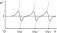
\includegraphics[scale=1]{figures/ch_20/fig_20_5.pdf}
			% \caption[]{}
            \caption[]{Behaviour of function \eqref{eq:20_22} when the friction of emission is disregarded (dashed line) and when is considered (solid line).}
			\label{fig:20_5}
		\end{center}
	\end{minipage}
	\hfill{ }%space{-0.05cm}
	\begin{minipage}[t]{0.48\linewidth}
		\begin{center}
			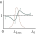
\includegraphics[scale=1]{figures/ch_20/fig_20_6.pdf}
            % \caption[]{}
			\caption[]{Square root of \fig{20_5} in terms of $\lambda_0$. The dash curve shows how the coefficient of absorption of light by a substance changes.}
			\label{fig:20_6}
		\end{center}
	\end{minipage}
\vspace{-0.4cm}
\end{figure}

Passing over from $n^2$ to $n$ and from $\omega$ to $\lambda_0$, we get the curve shown in \fig{20_6} (the figure gives only a portion of the curve in the region of one of the resonance wavelengths).
The dash curve in this figure shows how the coefficient of absorption of light by a substance changes (see the following section).
Segment $3$-$4$ is similar to the curve shown in \fig{20_1}.
Segments $1$-$2$ and $3$-$4$ correspond to normal dispersion ($\diffin{n}{\lambda_0}<0$).
On segment $2$-$3$, the dispersion is anomalous ($\diffin{n}{\lambda_0}>0$).
In region $1$-$2$, the refractive index is less than unity, hence, the phase velocity of the wave exceeds $c$.
This circumstance does not contradict the theory of relativity, which is based on the statement that the velocity of transmitting a signal cannot exceed $c$.
In the preceding section, we found that it is impossible to transmit a signal with the aid of an ideally monochromatic wave.
Energy (\ie, a signal) is transmitted with the aid of a not completely monochromatic wave (wave packet), however, with a velocity equal to the group velocity determined by \eqn{20_17}.
In the region of normal dispersion, $\diffin{n}{\lambda}>0$ ($\deriv{n}$ and $\deriv{\lambda}$ have different signs, while
$\diffin{n}{\lambda}<0$), so that although $v>c$, the group velocity is less than $c$.
In the region of anomalous dispersion, the concept of group velocity loses its meaning (the absorption is very great).
Therefore, the value of $u$ calculated by \eqn{20_17} will not characterize the rate of energy transmission.
The relevant calculations give a value less than $c$ for the velocity of energy transmission in this case too.

\section{Absorption of Light}\label{sec:20_4}

When a light wave passes through a substance, part of the wave energy is spent for producing oscillations of the electrons.
This energy is partly returned to the radiation in the form of the secondary wavelets set up by the electrons; it is partly transformed, however, into the energy of motion of the atoms, \ie, into the internal energy of the substance.
This is the reason why the intensity of light transmitted through a substance diminishes---light is absorbed in the substance.
The forced oscillations of the electrons and therefore the absorption of light become especially intensive at the resonance frequency (see the dash absorption curve in \fig{20_6}).

Experiments show that the intensity of light when it passes through a substance diminishes according to the exponential law
\begin{equation}\label{eq:20_23}
	I = I_0 e^{-\varkappa l}.
\end{equation}

\noindent
Here, $I_0$ is the intensity of light at the entrance to the absorbing layer (on its boundary or at a certain place inside the substance), $l$ is the thickness of the layer, and $\varkappa$ is the constant depending on the properties of the absorbing substance and called the \textbf{absorption coefficient}.

Equation \eqref{eq:20_23} is known as \textbf{Bouguer's law}\footnote{Also known as the Beer-Lambert law or Beer-Lambert-Bouguer law.} [in honour of the French scientist Pierre Bouguer (1698-1758)].

Differentiation of \eqn{20_23} yields
\begin{equation}\label{eq:20_24}
	\deriv{I} = - \varkappa I_0 e^{-\varkappa l}\, \deriv{l} = -\varkappa I\, \deriv{l}.
\end{equation}

\noindent
It follows from this expression that the decrement of the intensity along the path $\deriv{l}$ is proportional to the length of this path and to the value of the intensity itself.
The absorption coefficient is the constant of proportionality.

Inspection of \eqn{20_23} shows that when $l=1/\varkappa$, the intensity $I$ is $1/e$-th of $I_0$.
Thus, the absorption coefficient is a quantity inversely proportional to the thickness of the layer that reduces the intensity of light passing through it to $1/e$-th of its initial value.

The absorption coefficient depends on the wavelength $\lambda$ (or the frequency $\omega$).
The absorption coefficient of a substance whose atoms or molecules do not virtually act on one another (gases and metal vapours at a low pressure) is close to zero for most wavelengths.
It displays sharp maxima (\fig{20_7}) only for very narrow spectral regions (having a width of several hundredths of an angstrom).
These maxima correspond to the resonance frequencies of oscillations of the electrons inside the atoms.
For polyatomic molecules, frequencies corresponding to the oscillations of the atoms inside the molecules are also detected.
Since the masses of atoms are tens of thousands of times greater than the mass of an electron, the molecular frequencies are much smaller than the atomic ones---they are in the infrared region
of the spectrum.

Gases at high pressures, and also liquids and solids produce broad absorption bands (\fig{20_8}).
As the pressure of gases is increased, the absorption maxima, which are initially very narrow (see \fig{20_7}), expand more and more, and at high pressures the absorption spectrum of gases approaches those of liquids.
This fact indicates that the expansion of the absorption bands is the result of the atoms interacting with one another.

\begin{figure}[t]
	\begin{minipage}[t]{0.56\linewidth}
		\begin{center}
			\includegraphics[scale=1]{figures/ch_20/fig_20_7.pdf}
			% \caption[]{}
            \caption[]{The absorption coefficient of a substance whose atoms or molecules do not virtually act on one another (gases and metal vapours at a low pressure) is close to zero for most wavelengths. It displays sharp maxima (\fig{20_7}) only for very narrow spectral regions (having a width of several hundredths of an angstrom). These maxima correspond to the resonance frequencies of oscillations of the electrons inside the atoms. The molecular frequencies are in the infrared region of the spectrum.}
			\label{fig:20_7}
		\end{center}
	\end{minipage}
	\hfill{ }%space{-0.05cm}
	\begin{minipage}[t]{0.40\linewidth}
		\begin{center}
			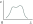
\includegraphics[scale=1]{figures/ch_20/fig_20_8.pdf}
            % \caption[]{}
			\caption[]{Broad absorption bands of gases at high pressures (also liquids and solids). As the pressure of gases is increased, the absorption maxima expand and at high pressures the absorption spectrum of gases approaches those of liquids. This indicates that the expansion of the absorption bands is the result of the atoms interacting with one another.}
			\label{fig:20_8}
		\end{center}
	\end{minipage}
\vspace{-0.4cm}
\end{figure}

Metals are virtually opaque for light ($\varkappa$ for them has a value of the order of \SI{e6}{\per\metre}; for comparison we shall point out that for glass $\varkappa\approx\SI{1}{\per\metre}$).
This is due to the presence of free electrons in metals.
The action of the electric field of a light wave causes the free electrons to come into motion---fast-varying currents attended by the liberation of Lenz-Joule heat are produced in the metal.
As a result, the energy of the light wave rapidly diminishes and transforms into the internal energy of the metal.

\section{Scattering of Light}\label{sec:20_5}

From the classical viewpoint, the process of scattering of light consists in that light passing through a substance causes the electrons
in the atoms to oscillate.
The oscillating electrons produce secondary wavelets that propagate in all directions.
This phenomenon should seem to result in the scattering of light in all conditions.
The secondary wavelets, however, are coherent, so that their mutual interference must be taken into consideration.

The relevant calculations show that in a homogeneous medium the secondary wavelets completely destroy one another in all directions except for that of propagation of the primary wave.
Therefore, no redistribution of the light by directions, \ie, scattering of the light, occurs.

The secondary wavelets do not destroy one another in side directions only when light propagates in a non-homogeneous medium.
The light waves become diffracted on the non-homogeneities of the medium and produce a diffraction pattern characterized by a quite uniform distribution of the intensity between all directions.
Such diffraction on fine non-homogeneities is called the \textbf{scattering of light}.

Media having a clearly expressed optical non-homogeneity are known as \textbf{turbid media}.
They include (1) smoke, \ie, a suspension of very minute solid particles in a gas, (2) fogs and mists-suspensions of very minute liquid droplets in gases, (3) suspensions formed by solid particles in the bulk of a liquid, (4) emulsions, \ie, suspensions of very minute droplets of one liquid in another one that does not dissolve the first liquid (an example of an emulsion is milk, which is a suspension of droplets of fat in water), and (5) solids such as mother-of-pearl, opals, and milk glass.

Light scattered on particles whose size is considerably smaller than the length of a light wave becomes partly polarized.
The explanation is that the oscillations of the electrons produced by the scattered light beam occur in a plane at right angles to the beam (\fig{20_9}).
The oscillations of the vector $\vec{E}$ in a secondary wavelet occur in a plane passing through the direction of oscillations of the charges (see \fig{15_6}).
Therefore, the light scattered by the particles in directions normal to the beam will be completely polarized.
The scattered light is polarized only partly in directions that make an angle other than a right one with the beam.

\begin{figure}[t]
	\begin{center}
		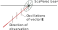
\includegraphics[scale=1]{figures/ch_20/fig_20_9.pdf}
		% \caption[]{}
        \caption[]{The light scattered by the particles in directions normal to the beam will be completely polarized. The scattered light is polarized only partly in directions that make an angle other than a right one with the beam.}
		\label{fig:20_9}
	\end{center}
	\vspace{-0.8cm}
\end{figure}

As a result of scattering of the light in side directions, the intensity in the direction of its propagation diminishes more rapidly than when only absorption occurs.
Consequently, for a turbid substance, \eqn{20_23} must contain the coefficient $\varkappa'$ due to scattering in addition to the absorption coefficient $\varkappa$:
\begin{equation}\label{eq:20_25}
	I = I_0 e^{-(\varkappa+\varkappa')l}.
\end{equation}

\noindent
The constant $\varkappa'$ is called the \textbf{extinction coefficient}.

If the dimensions of the non-homogeneities are small in comparison with the length of a light wave (not over $\sim 0.1\lambda$), then the
intensity of the scattered light $l$ is proportional to the fourth power of the frequency or is inversely proportional to the fourth power of the wavelength:
\begin{equation}\label{eq:20_26}
	I \propto \omega^4 \propto \frac{1}{\lambda^4}.
\end{equation}

\noindent
This relation is known as \textbf{Rayleigh's law} after the British physicist John Rayleigh (1842-1919).
It is easy to understand its origin if we take into account that the radiant power of an oscillating charge is proportional to the fourth power of the frequency and, consequently, is inversely proportional to the fourth power of the wavelength [see expression \eqref{eq:15_46}].

If the dimensions of the non-homogeneities are comparable with the length of a wave, then the electrons at different spots on the non-homogeneities oscillate with an appreciable phase shift.
This circumstance makes the phenomenon more complicated and leads to other regularities---the intensity of the scattered light becomes proportional to only the square of the frequency (inversely proportional to the square of the wavelength).

It is simple to observe the manifestation of law \eqref{eq:20_26} by passing a beam of white light through a vessel with a turbid liquid (\fig{20_10}).
Owing to scattering, the trace of the beam in the liquid is seen very well from a side.
Since short light waves are scattered to a much greater extent than the long ones, the trace seems to be bluish.
The beam passing through the liquid is enriched with long-wave radiation and forms a reddish-yellow spot on screen Sc instead of a white one.
If we put polarizer P at the entrance of the beam to the vessel, we shall find that the intensity of the scattered light in different directions perpendicular to the initial beam is not the same.
The directivity of dipole emission (see \fig{15_7}) results in the fact that in the directions coinciding with the plane of oscillations of the primary beam, the intensity of the scattered light virtually equals zero, while in the directions perpendicular to the plane of the oscillations, the intensity of the scattered light is maximum.
By turning the polarizer around the direction of the primary beam, we shall observe alternate amplification and attenuation of the light scattered in the given direction.

\begin{figure}[t]
	\begin{center}
		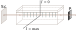
\includegraphics[scale=1]{figures/ch_20/fig_20_10.pdf}
		% \caption[]{}
        \caption[]{A beam of white light passing through a vessel with a turbid liquid. The beam passing through the liquid is enriched with long-wave radiation and forms a reddish-yellow spot on screen Sc instead of a white one. With a polarizer P at the entrance of the beam to the vessel, we shall find that the intensity of the scattered light in different directions perpendicular to the initial beam is not the same.}
		\label{fig:20_10}
	\end{center}
	\vspace{-0.8cm}
\end{figure}

Even liquids and gases carefully purified of foreign admixtures and impurities scatter light to some extent.
The Soviet physicist Leonid Mandelshtam (1879-1944) and the Polish physicist Marian Smoluchowski (1872-1917) established that the appearance of the optical non-homogeneities is due in this case to fluctuation of the density (\ie, deviations of the density from its mean value observed within the confines of small volumes).
These fluctuations are produced by chaotic motion of the molecules of the substance; therefore, the scattering of light due to them is called \textbf{molecular}.

Molecular scattering explains the light blue colour of the sky.
The places of compression and rarefaction of the air continuously appearing in the atmosphere owing to the random motion of its molecules scatter sunlight.
According to law \eqref{eq:20_26}, the light blue and blue rays are scattered to a greater extent than the yellow and red ones, the result being the light blue colour of the sky.
When the Sun is low above the horizon, the rays propagating directly from it pass through a scattering medium of great thickness, and as a result they are enriched with waves of greater lengths.
This is why the sky at sunrise and sunset has red tints.

There are especially favourable conditions for  the appearance of considerable density fluctuations near the critical state of a substance (at the critical point $\diffin{p}{V}= 0$; see Sec. 15.4 of Vol. I).
These fluctuations result in intensive scattering of light such that a glass ampule with the substance seems to be absolutely black when looked through.
This phenomenon is known as \textbf{critical opalescence}.

\section{The Vavilov-Cerenkov Effect}\label{sec:20_6}

In 1934, the Soviet physicist Pavel Cerenkov (born 1904), working under the supervision of Sergei Vavilov (1891-1951), discovered a special kind of glow of liquids under the action of radium gamma-rays.
Vavilov advanced the correct assumption that the fast electrons produced by the gamma-rays are the source of the radiation.
This phenomenon was named the \textbf{Vavilov-Cerenkov effect}.
Its complete theoretical explanation was given in 1937 by the Soviet physicists Igor Tamm (1895-1971) and Ilya Frank (born 1908)\footnote{In 1958, Cerenkov, Tamm, and Frank were awarded a Nobel prize for their work.}.

According to the electromagnetic theory, a charge moving uniformly emits no electromagnetic waves (see \sect{15_6}).
As Tamm and Frank showed, however, this holds only if the velocity $v$ of a charged particle does not exceed the phase velocity $c/n$ of electromagnetic waves in the medium in which the particle is moving.
A particle emits electromagnetic waves even when travelling uniformly provided that $v>c/n$.
The particle actually loses energy on radiation owing to which it travels with a negative acceleration.
This acceleration is not the cause (as when $v<c/n$), but a consequence of radiation.
If the loss of energy at the expense of radiation were replenished in some way or other, a particle travelling uniformly with the velocity $v>c/n$ would nevertheless be a source of radiation.

The Vavilov-Cerenkov effect was observed experimentally for electrons, protons, and mesons travelling in liquid and solid media.

Vavilov-Cerenkov radiation has a light blue colour because short waves predominate in it.
The most characteristic feature of this radiation is the fact that it is emitted not in all directions, but only along the generatrices of a cone whose axis coincides with the direction
of velocity of the relevant particle (\fig{20_11}).
The angle $\theta$ between the directions of propagation of the radiation and the velocity vector of a particle is determined by the equation
\begin{equation}\label{eq:20_27}
	\cos\theta = \frac{c/n}{v} = \frac{c}{nv}.
\end{equation}

\begin{figure}[t]
	\begin{center}
		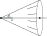
\includegraphics[scale=1]{figures/ch_20/fig_20_11.pdf}
		% \caption[]{}
        \caption[]{Vavilov-Cerenkov radiation most characteristic feature is that it is emitted not in all directions, but only along the generatrices of a cone whose axis coincides with the direction of velocity of the relevant particle. The angle $\theta$ is formed between the directions of propagation of the radiation and the velocity vector of a particle.}
		\label{fig:20_11}
	\end{center}
	\vspace{-0.8cm}
\end{figure}

The Vavilov-Cerenkov effect finds widespread application in experimental equipment.
In the so-called Cerenkov counters, a light pulse produced by a fast charged particle is transformed with the aid of a photomultiplier\footnote{By a photomultiplier is meant an electronic multiplier whose first electrode (a photocathode) is capable of emitting electrons under the action of light.} into a current pulse.
To make such a counter function, the energy of a particle must exceed the threshold value determined by the condition $v = c/n$.
Therefore, Cerenkov counters make it possible not only to register particles, but also to assess their energy.
It is even possible to determine the angle $\theta$ between the direction of a flash and the velocity of the particle.
This allows us to use \eqn{20_27} to calculate the velocity (and, consequently, also the energy) of a particle.
